\documentclass[]{article}

  \title{Regressão Exponencial\newline\large Otimização}
  \author{Hugo Veríssimo 75692\newline Lara Pereira 75695\newline Miriam
Marques 75556}
  \date{\today}
  


\newcommand{\logo}{./ualg.png}
\newcommand{\cover}{./cover3.jpg}
\newcommand{\iblue}{2b4894}
\newcommand{\igray}{d4dbde}
\usepackage{amsmath}
\numberwithin{equation}{subsection}
\usepackage[hidelinks]{hyperref}

\usepackage{listings}
\lstdefinestyle{mystyle}{
    basicstyle=\ttfamily, % Set the font to a monospaced (typewriter) font
    breaklines=true, % Allow line breaks
    keywordstyle=\color{blue}, % Set the color of keywords
    commentstyle=\color{green!40!black}, % Set the color of comments
    numbers=left, % Display line numbers
    numberstyle=\tiny\color{gray}, % Set the style of line numbers
    frame=single, % Draw a frame around the code
    rulecolor=\color{black!30}, % Set the frame color
    backgroundcolor=\color{gray!10}, % Set the background color
    captionpos=b, % Position of the caption (b for bottom)
    showstringspaces=false % Don't emphasize spaces in strings
}

\lstset{style=mystyle} % Set the default style to the one you defined

% /\ eu meti para mudar a fonte do codigo ig


% % % packages -----------------------------------------------------------------------------------
\usepackage[portuges]{babel}
\usepackage[utf8]{inputenc}
\usepackage{amsmath}
\usepackage{amssymb}
\usepackage{array}
\usepackage{booktabs}
\usepackage{calc}
\usepackage{eso-pic}
\usepackage{fancyhdr}
\usepackage{fontspec}
\usepackage[left = 2.5cm, right = 2.5cm, top = 1cm, bottom = 1cm, includeheadfoot]{geometry}
\usepackage{graphicx}
\usepackage{lastpage}
\usepackage{multirow}
\usepackage{tabularx} 
\usepackage{tikz}
\usepackage{titlesec}
\usepackage{xcolor, colortbl}

% % % settings -----------------------------------------------------------------------------------

% % custom colors
\definecolor{iblue}{HTML}{\iblue}
\definecolor{igray}{HTML}{\igray}

% definition of pagename
%\newcommand\pagename{Page}
\renewcommand{\contentsname}{Índice}

% % fonts 
\defaultfontfeatures{Mapping = tex-text}
\setmainfont[BoldFont = Lato-Bold.ttf, ItalicFont = Lato-Italic.ttf, BoldItalicFont = Lato-BoldItalic.ttf]{Lato-Regular.ttf}
\newfontfamily\headingfont[ItalicFont = Lato-BlackItalic.ttf]{Lato-Black.ttf}


% % sections
\titleformat{\section}{\color{iblue}\headingfont\Large\bfseries}{\thesection}{1em}{}[\titlerule]
\titleformat{\subsection}{\color{iblue}\headingfont\large\bfseries}{\thesubsection}{1em}{}
\titleformat{\subsubsection}{\color{iblue}\headingfont\bfseries}{\thesubsubsection}{1em}{}

% % misc
\setlength{\parindent}{0em} 
\linespread{1.3}
\raggedright
\newcolumntype{C}{>{\centering\arraybackslash}X}


% % % custom titlepage ----------------------------------------------------------------------------
\newcommand\BackgroundPic{%
	\put(0,0){%
		\parbox[b][\paperheight]{\paperwidth}{%
			\vfill
			\centering
			\includegraphics[width=\paperwidth,height=\paperheight]{\cover}%
			\vfill
}}}

\makeatletter

% pagestyle titlepage
\fancypagestyle{customtitle}{
	\lhead{}
	\chead{}
	\rhead{}
	\makeatother
	\lfoot{}
	\cfoot{}
	\rfoot{\includegraphics[scale=0.3]{\logo}}
}


% titlepage
\renewcommand{\maketitle}{
	\thispagestyle{customtitle}
	\AddToShipoutPicture*{\BackgroundPic}
	\ClearShipoutPicture
	
	\phantom{a}\hfill
	\vspace{15cm}
	
	\begin{tabular}[l]{@{}p{\textwidth}@{}}
		\color{iblue}\headingfont\LARGE\@title\\[1em]
		\color{iblue}\headingfont\large\@author\\[1em]
		\color{iblue}\headingfont\small\@date\\[1em]
	\end{tabular}
	
	
	
	\clearpage
}
\makeatother

% % % header and footer ---------------------------------------------------------------------------
\pagestyle{fancy}
\lhead{}
\chead{}
\rhead{ \includegraphics[scale=0.2]{\logo}}
\makeatother
\newlength{\myheight}
\lfoot{}
\cfoot{}
\rfoot{\pagename~\thepage \hspace{1pt} / \pageref{LastPage}}
\renewcommand\headrulewidth{0pt}
\renewcommand\footrulewidth{0pt}

% % % shading for code ---------------------------------------------------------------------------
\usepackage{color}
\usepackage{fancyvrb}
\newcommand{\VerbBar}{|}
\newcommand{\VERB}{\Verb[commandchars=\\\{\}]}
\DefineVerbatimEnvironment{Highlighting}{Verbatim}{commandchars=\\\{\}}
% Add ',fontsize=\small' for more characters per line
\usepackage{framed}
\definecolor{shadecolor}{RGB}{248,248,248}
\newenvironment{Shaded}{\begin{snugshade}}{\end{snugshade}}
\newcommand{\KeywordTok}[1]{\textcolor[rgb]{0.13,0.29,0.53}{\textbf{#1}}}
\newcommand{\DataTypeTok}[1]{\textcolor[rgb]{0.13,0.29,0.53}{#1}}
\newcommand{\DecValTok}[1]{\textcolor[rgb]{0.00,0.00,0.81}{#1}}
\newcommand{\BaseNTok}[1]{\textcolor[rgb]{0.00,0.00,0.81}{#1}}
\newcommand{\FloatTok}[1]{\textcolor[rgb]{0.00,0.00,0.81}{#1}}
\newcommand{\ConstantTok}[1]{\textcolor[rgb]{0.00,0.00,0.00}{#1}}
\newcommand{\CharTok}[1]{\textcolor[rgb]{0.31,0.60,0.02}{#1}}
\newcommand{\SpecialCharTok}[1]{\textcolor[rgb]{0.00,0.00,0.00}{#1}}
\newcommand{\StringTok}[1]{\textcolor[rgb]{0.31,0.60,0.02}{#1}}
\newcommand{\VerbatimStringTok}[1]{\textcolor[rgb]{0.31,0.60,0.02}{#1}}
\newcommand{\SpecialStringTok}[1]{\textcolor[rgb]{0.31,0.60,0.02}{#1}}
\newcommand{\ImportTok}[1]{#1}
\newcommand{\CommentTok}[1]{\textcolor[rgb]{0.56,0.35,0.01}{\textit{#1}}}
\newcommand{\DocumentationTok}[1]{\textcolor[rgb]{0.56,0.35,0.01}{\textbf{\textit{#1}}}}
\newcommand{\AnnotationTok}[1]{\textcolor[rgb]{0.56,0.35,0.01}{\textbf{\textit{#1}}}}
\newcommand{\CommentVarTok}[1]{\textcolor[rgb]{0.56,0.35,0.01}{\textbf{\textit{#1}}}}
\newcommand{\OtherTok}[1]{\textcolor[rgb]{0.56,0.35,0.01}{#1}}
\newcommand{\FunctionTok}[1]{\textcolor[rgb]{0.00,0.00,0.00}{#1}}
\newcommand{\VariableTok}[1]{\textcolor[rgb]{0.00,0.00,0.00}{#1}}
\newcommand{\ControlFlowTok}[1]{\textcolor[rgb]{0.13,0.29,0.53}{\textbf{#1}}}
\newcommand{\OperatorTok}[1]{\textcolor[rgb]{0.81,0.36,0.00}{\textbf{#1}}}
\newcommand{\BuiltInTok}[1]{#1}
\newcommand{\ExtensionTok}[1]{#1}
\newcommand{\PreprocessorTok}[1]{\textcolor[rgb]{0.56,0.35,0.01}{\textit{#1}}}
\newcommand{\AttributeTok}[1]{\textcolor[rgb]{0.77,0.63,0.00}{#1}}
\newcommand{\RegionMarkerTok}[1]{#1}
\newcommand{\InformationTok}[1]{\textcolor[rgb]{0.56,0.35,0.01}{\textbf{\textit{#1}}}}
\newcommand{\WarningTok}[1]{\textcolor[rgb]{0.56,0.35,0.01}{\textbf{\textit{#1}}}}
\newcommand{\AlertTok}[1]{\textcolor[rgb]{0.94,0.16,0.16}{#1}}
\newcommand{\ErrorTok}[1]{\textcolor[rgb]{0.64,0.00,0.00}{\textbf{#1}}}
\newcommand{\NormalTok}[1]{#1}

\newtheorem{theorem}{Teorema}[section]
\newtheorem{corollary}{Corolário}[theorem]
\newtheorem{lemma}[theorem]{Lema}
\newtheorem{definition}{Definição}[section]
\newenvironment{proof}{\paragraph{Demonstração:}}{\hfill$\square$}

\setlength{\headheight}{18.10197pt}

\usepackage{ragged2e}
\justifying

\begin{document}



\maketitle
\tableofcontents
\addcontentsline{toc}{section}{Índice}
\clearpage

\section{Introdução}

A função exponencial tem uma presença constante na matemática pura e
aplicada, levando o famoso matemático W. Rudin a referir que a função
exponencial é a ``função mais importante da matemática'' \cite{WR87}.
Esta possui aplicações em áreas como: economia, probabilidades,
estatística, biologia, física, medicina, engenharia, entre outras.

\(\ \)

O crescimento populacional, analisado geralmente através da construção e
interpretação de gráficos de dados macroeconómicos, pode ser explicado
através das propriedades algébricas e gráficas das funções exponenciais
e logarítmicas para o cálculo e interpretação de taxas de crescimento
populacional através de séries temporais.

\(\ \)

O número de Euler é também muito aplicado nas finanças, principalmente
em cálculos de juros compostos, onde a riqueza cresce a uma taxa
definida ao longo do tempo \cite{WK23}.

\(\ \)

Um comum problema computacional é o do cálculo da solução para problemas
de mínimos quadrados, que possui grande importância numa ampla gama de
campos que vão desde a álgebra linear até à econometria e otimização. O
grande leque de aplicações em diversas áreas confere à função
exponencial um estatuto muito importante no campo matemático pelo que a
mesma será utilizada como título exemplificativo para a resolução de
sistemas não lineares de equações no presente trabalho. Neste, iremos
apresentar algoritmos numericamente estáveis e computacionalmente
eficientes para calcular a solução do problema de mínimos quadrados.

\(\ \)

Dado um conjunto de pontos observados a função exponencial em conjunto
com o método dos mínimos quadrados visa encontrar os parâmetros de um
determinado modelo matemático de forma a minimizar a soma dos quadrados
entre os valores observados e os valores previstos pelo modelo ajustado.

\(\ \)

A descoberta do vetor de parâmetros que minimiza a função objetivo pode
então ser realizada com recurso a várias técnicas. No presente trabalho
serão abordadas duas das mesmas, a decomposição QR e o método de
Levenberg-Marquardt. De forma a avaliar e comparar a estabilidade e
eficiência dos mesmos, foram analisados conceitos teóricos e resultados
numéricos provenientes de algoritmos criados.

\(\ \)

A decomposição QR foi considerada um dos 10 algoritmos com maior
influência no desenvolvimento e na prática da ciência e da engenharia no
século XX \cite{BAC00}.

\(\ \)

Contudo, como parte da revolução industrial, a produção industrial foi
otimizada de forma a ser mais inteligente e automatizada. A crescente
complexidade da produção industrial aumenta então os requisitos de
precisão e velocidade \cite{XHHCBJ23}.

Métodos de resolução de sistemas não lineares como o de
Levenberg-Marquardt e evoluções destes são essenciais para assegurar a
satisfação da crescente procura por uma otimização mais eficiente.

\newpage
\section{Decomposição QR}

A decomposição QR é utilizada para a resolução de sistemas
sobredeterminados, através do método dos mínimos quadrados. Assim sendo,
esta pode ser utilizada para a resolução do nosso problema.

A decomposição QR tem como objetivo expressar uma matriz
\(A\in \mathbb{M}_{m,n} (\mathbb{R})\) no produto de duas matrizes, uma
ortogonal \((Q)\) e outra triangular superior \((R)\). Assim, a
decomposição de A é tal que: \begin{equation}
A=QR
\end{equation} onde \(Q\in \mathbb{M}_{m,n} (\mathbb{R})\) é uma matriz
cujas colunas formam uma base ortonormada para o espaço das colunas de A
(isto é, \(Q^T Q = I_n\)) e \(R\in \mathbb{M}_{n,n} (\mathbb{R})\) é uma
matriz invertível, triangular superior com entradas diagonais positivas.

Existem diversos métodos para executar a decomposição QR, sendo um deles
o processo de Gram-Schmidt, que constitui uma técnica de
ortonormalização. Note-se que para além dessa técnica existem outras
mais estáveis numericamente, como é o caso do algoritmo de Householder
\cite{GASMK08}.

\subsection{Processo de Ortonormalização de Gram-Schmidt}

A aplicação do processo de ortonormalização de Gram-Schmidt requer a
utilização dos vetores que correspondem às colunas da matriz A.
\begin{equation}
A=[a_1|a_2|...|a_n]
\end{equation} Dois passos essenciais do processo referido são a
ortogonalização e a normalização. A realização da ortogonalização tem
como intuito a transformação do conjunto de vetores linearmente
independentes num conjunto ortogonal, onde cada vetor é ortogonal
(perpendicular) aos outros. A normalização transforma este conjunto
ortogonal num conjunto ortonormal, isto é, cada vetor possui norma igual
a 1.

Então \cite{IY07}, \begin{multline}
\begin{aligned}
& v_1 = a_1, && q_1 = \frac{v_1}{\|v_1\|_2} \\
& v_2 = a_2 - (q_1^T \cdot a_2) q_1, && q_2 = \frac{v_2}{\|v_2\|_2} \\
& v_3 = a_3 - (q_1^T \cdot a_3) q_1 - (q_2^T \cdot a_3) q_2, && q_3 = \frac{v_3}{\|v_3\|_2} \\
& \vdots && \hspace{7.65cm} \\
& v_n = a_n - (q_1^T \cdot a_n) q_1 - \ldots - (q_{n-1}^T \cdot a_n) q_{n-1}, && q_n = \frac{v_n}{\|v_n\|_2}
\end{aligned}
\end{multline}

\subsection{Algoritmo de Gram-Schmidt Clássico}

Note-se que após o processo de ortogonalização e normalização, obtém-se
a decomposição QR da matriz A:

\begin{equation}
A = [a_1| a_2|...| a_n] = [q_1| q_2|...| q_n]
\begin{bmatrix}
\|v_1\|_2 & q_1^T\cdot a_2 &...& q_1^T\cdot a_n \\
0 & \|v_2\|_2 &...& q_2^T\cdot a_n \\
\vdots & \vdots & \ddots &\vdots \\
0 & 0 &...& \|v_n\|_2 
\end{bmatrix}
= QR
\end{equation}

\newpage
\subsubsection{Implementação em Python}

As ideias acima apresentadas podem ser sintetizadas através do seguinte
algoritmo:

\begin{Shaded}
\begin{Highlighting}[]
\ImportTok{import}\NormalTok{ numpy }\ImportTok{as}\NormalTok{ np}

\KeywordTok{def}\NormalTok{ QRdecomposition\_Gram\_Schmidt(A):}
    \CommentTok{"""}
\CommentTok{    entrada:}
\CommentTok{        A {-} matriz a decompor}
\CommentTok{    saída:}
\CommentTok{        Q {-} matriz ortogonal}
\CommentTok{        R {-} matriz triangular superior}
\CommentTok{    """}
\NormalTok{    q }\OperatorTok{=}\NormalTok{ [] }\CommentTok{\#sera a lista de colunas de Q}
\NormalTok{    R }\OperatorTok{=}\NormalTok{ np.zeros((}\BuiltInTok{len}\NormalTok{(A[}\DecValTok{0}\NormalTok{]), }\BuiltInTok{len}\NormalTok{(A[}\DecValTok{0}\NormalTok{])), dtype}\OperatorTok{=}\BuiltInTok{float}\NormalTok{) }\CommentTok{\# matriz R, preenchida de zeros}

    \CommentTok{\# percorrer as colunas da matriz A}
    \ControlFlowTok{for}\NormalTok{ i }\KeywordTok{in} \BuiltInTok{range}\NormalTok{(}\BuiltInTok{len}\NormalTok{(np.transpose(A))):}
\NormalTok{        ai }\OperatorTok{=}\NormalTok{ np.transpose(A)[i] }\CommentTok{\#ai = coluna i de A}

\NormalTok{        projecoes }\OperatorTok{=} \DecValTok{0} \CommentTok{\#a subtrair no calculo de vi}
        \CommentTok{\# percorrer as colunas Q ja calculadas}
        \ControlFlowTok{for}\NormalTok{ n }\KeywordTok{in} \BuiltInTok{range}\NormalTok{(}\BuiltInTok{len}\NormalTok{(q)):}
\NormalTok{            qn }\OperatorTok{=}\NormalTok{ q[n] }\CommentTok{\#qn = coluna n de Q, ja calculada, pelo que n \textless{} i}
\NormalTok{            R[n][i] }\OperatorTok{=}\NormalTok{ np.inner(qn,ai) }\CommentTok{\#calcular r\_\{n,i\}}
\NormalTok{            projecoes }\OperatorTok{+=}\NormalTok{ R[n][i]}\OperatorTok{*}\NormalTok{qn }\CommentTok{\#somar as projecoes a subtrair a ai}
        
        \CommentTok{\# calcular vi}
\NormalTok{        vi }\OperatorTok{=}\NormalTok{ ai }\OperatorTok{{-}}\NormalTok{ projecoes}

        \CommentTok{\# calcular r\_\{i,i\}: norma 2 de vi}
\NormalTok{        R[i][i] }\OperatorTok{=}\NormalTok{ np.sqrt(np.inner(vi,vi))}

        \CommentTok{\# calcular qi: normalizacao de vi}
\NormalTok{        qi }\OperatorTok{=}\NormalTok{ vi}\OperatorTok{/}\NormalTok{R[i][i]}
\NormalTok{        q.append(qi)}

    \CommentTok{\# converter q numa matriz (Q\textquotesingle{}) e transpor}
\NormalTok{    Q }\OperatorTok{=}\NormalTok{ np.transpose(np.vstack(q))}

    \ControlFlowTok{return}\NormalTok{ Q,R}
\end{Highlighting}
\end{Shaded}

\newpage
\subsection{Regressão Exponencial} \label{exp_aplicado_qr}

Pretende-se utilizar a decomposição QR para estimar os parâmetros que
otimizam, no sentido dos mínimos quadrados, uma função exponencial
\(y(x)\): \begin{equation}
y(x)=\beta_{0} e^{\beta_{1}x}
\end{equation}

\subsubsection{Linearização do Problema}

Todavia, a função \(y(x)\) não é linear pelo que não é possível obter a
matriz \(A\), impossibilitando a aplicação da decomposição QR. Por esse
motivo, terão que ser realizadas transformações na expressão com o
objetivo de linearizar a mesma.

Aplicando logaritmos, \begin{equation}
ln(y(x))=ln(\beta_{0} e^{\beta_{1}x})
\end{equation}

Através das propriedades dos logaritmos,
\begin{equation} \label{eq:exp_linearizada}
ln(y(x))=ln(\beta_{0}) + \beta_{1}x
\end{equation}

Assumindo \(P(x)=ln(y(x))\), \(a_0=ln(\beta_{0})\) e \(a_1=\beta_{1}\),
tem-se \begin{equation}
P(x)=a_0 + a_1x
\end{equation}

Uma vez obtida a função \(y(x)\) como combinação linear de funções, a
fase de linearização está completa pelo que se pode proceder à aplicação
da decomposição QR.

\subsubsection{Resolução do Problema}

A descoberta dos parâmetros passa pela resolução do sistema \(Ax=b\),
onde \(A\) é a matriz de coeficientes dos parâmetros a estimar do
sistema de equações, \(x\) é o vetor solução dos parâmetros a estimar e
\(b\) é o vetor que contém as variáveis resposta do sistema de equações.

Aplicando a decomposição QR à matriz \(A\) obtém-se \(QR=A\), pelo que
podem ser efetuadas as seguintes equivalências matriciais:
\begin{equation}
Ax=b \Leftrightarrow QRx=b \Leftrightarrow Q^TQRx=Q^Tb \Leftrightarrow IRx=Q^Tb \Leftrightarrow Rx=Q^Tb
\end{equation} Sendo assim, a resolução do sistema de equações \(Ax=b\)
passa pela resolução do sistema \(Rx=Q^Tb\), em que \(R\) é a matriz
triangular superior proveninente da decomposição QR e \(Q^T\) é a
transposta da matriz \(Q\), também proveniente da decomposição QR,
obtendo desta forma, o vetor \(x\) dos parâmetros.

Tem-se então: \begin{equation} \label{eq:exp_qr1}
Ax=b
\quad \Leftrightarrow \quad
\begin{bmatrix}
1 & x_1 \\ 1 & x_2 \\ \vdots & \vdots \\ 1 & x_n
\end{bmatrix}
\begin{bmatrix}
ln(\beta_0) \\ \beta_1
\end{bmatrix}
=
\begin{bmatrix}
ln(y_1) \\ ln(y_2) \\ \vdots \\ ln(y_n)
\end{bmatrix}
\quad \Rightarrow \quad
R
\begin{bmatrix}
ln(\beta_0) \\ \beta_1
\end{bmatrix}
=
Q^T
\begin{bmatrix}
ln(y_1) \\ ln(y_2) \\ \vdots \\ ln(y_n)
\end{bmatrix}
\end{equation}

\subsubsection{Exemplo - Regressão Exponencial: Problema Linearizado (QR)} \label{QR_exemplo}

Considere-se o seguinte exemplo ilustrativo da decomposição QR aplicada
a funções exponenciais.

Dado o seguinte conjunto de pontos acerca do Bangladesh \cite{Bang},
país de médio-baixo rendimento, pretende-se analisar o crescimento
exponencial do Rendimento Nacional Bruto (RNB) do mesmo de 2000 a 2019.
Os valores de \(x\) correspondem aos anos e os valores de \(y\) ao RNB
(em unidades por milhares de milhões de dólares).

\begin{table}[h]
\centering
\begin{tabular}{c|ccccccccccc}
\hline
\textbf{\(x_i\)} & 0 & 1 & 2 & 3 & 4 & 5 & 6 & 7 & 8 & 9 \\
\textbf{\(y_i\)} & 175.5 & 188.1 & 200.2 & 213.7 & 231.6 & 254.7 & 283.1 & 313.5 & 342.9 & 363.7  \\
\hline
\end{tabular}
\end{table}

\begin{table}[h]
\centering
\begin{tabular}{c|ccccccccccc}
\hline
\textbf{\(x_i\)} & 10 & 11 & 12 & 13 & 14 & 15 & 16 & 17 & 18 & 19 \\
\textbf{\(y_i\)} & 389.1 & 422.2 & 481.1 & 518.8 & 555.1 & 591.6 & 643.1 & 693.0  & 767.3 & 846.1 \\
\hline
\end{tabular}
\end{table}

A amostra de dados pode ser explicada pela função
\(y(x)=\beta_{0} e^{\beta_{1}x}\), pelo que se pretende obter o vetor de
parâmetros que minimiza a soma dos quadrados dos resíduos.

Primeiramente, tem que se proceder à linearização da nossa função. Visto
que a função \(y(x)\) é a mesma que foi utilizada na linearização
precedente então obter-se-á a expressão \ref{eq:exp_linearizada}. Uma
vez linearizada, os pontos referidos são aplicados à expressão obtida. A
dedução do vetor de parâmetros que contém \(\beta_{0}\) e \(\beta_{1}\)
passa pela resolução do sistema sobredeterminado \(Ax=b\)
(\ref{eq:exp_qr1}), através do seguinte algoritmo elaborado:

\begin{Shaded}
\begin{Highlighting}[]
\NormalTok{x }\OperatorTok{=} \BuiltInTok{list}\NormalTok{(}\BuiltInTok{range}\NormalTok{(}\DecValTok{19} \OperatorTok{+} \DecValTok{1}\NormalTok{))}
\NormalTok{y }\OperatorTok{=}\NormalTok{ [np.log(value) }\ControlFlowTok{for}\NormalTok{ value }\KeywordTok{in}\NormalTok{ [}\FloatTok{175.5}\NormalTok{, }\FloatTok{188.1}\NormalTok{, }\FloatTok{200.2}\NormalTok{, }\FloatTok{213.7}\NormalTok{, }\FloatTok{231.6}\NormalTok{, }\FloatTok{254.7}\NormalTok{, }\FloatTok{283.1}\NormalTok{,}
                                 \FloatTok{313.5}\NormalTok{, }\FloatTok{342.9}\NormalTok{, }\FloatTok{363.7}\NormalTok{, }\FloatTok{389.1}\NormalTok{, }\FloatTok{422.2}\NormalTok{, }\FloatTok{481.1}\NormalTok{, }\FloatTok{518.8}\NormalTok{,}
                                 \FloatTok{555.1}\NormalTok{, }\FloatTok{591.6}\NormalTok{, }\FloatTok{643.1}\NormalTok{, }\FloatTok{693.0}\NormalTok{, }\FloatTok{767.3}\NormalTok{, }\FloatTok{846.1}\NormalTok{]]}

\CommentTok{\# Ax = b; x = [ln(b0), b1]}
\NormalTok{A }\OperatorTok{=}\NormalTok{ np.column\_stack((np.ones(}\BuiltInTok{len}\NormalTok{(x)), x))}
\NormalTok{b }\OperatorTok{=}\NormalTok{ np.array(y).reshape(}\OperatorTok{{-}}\DecValTok{1}\NormalTok{, }\DecValTok{1}\NormalTok{)}
\NormalTok{Q, R }\OperatorTok{=}\NormalTok{ QRdecomposition\_Gram\_Schmidt(A)  }\CommentTok{\# QRx = b}
\NormalTok{Rx }\OperatorTok{=}\NormalTok{ np.dot(np.transpose(Q), b)  }\CommentTok{\# Rx = Qt*b}

\NormalTok{x }\OperatorTok{=}\NormalTok{ np.zeros(}\BuiltInTok{len}\NormalTok{(R))}
\ControlFlowTok{for}\NormalTok{ i }\KeywordTok{in} \BuiltInTok{range}\NormalTok{(}\BuiltInTok{len}\NormalTok{(R) }\OperatorTok{{-}} \DecValTok{1}\NormalTok{, }\OperatorTok{{-}}\DecValTok{1}\NormalTok{, }\OperatorTok{{-}}\DecValTok{1}\NormalTok{):}
\NormalTok{    x[i] }\OperatorTok{=}\NormalTok{ (Rx[i, }\DecValTok{0}\NormalTok{] }\OperatorTok{{-}}\NormalTok{ np.dot(R[i, i }\OperatorTok{+} \DecValTok{1}\NormalTok{:], x[i }\OperatorTok{+} \DecValTok{1}\NormalTok{:])) }\OperatorTok{/}\NormalTok{ R[i, i]}

\NormalTok{b0, b1 }\OperatorTok{=}\NormalTok{ np.exp(x[}\DecValTok{0}\NormalTok{]), x[}\DecValTok{1}\NormalTok{]}
\NormalTok{b0, b1}
\end{Highlighting}
\end{Shaded}

\begin{verbatim}
## (171.00724094657875, 0.08356097087277026)
\end{verbatim}

Assim sendo, a função que minimiza os quadrados dos resíduos, de acordo
com a decomposição QR, é dada por aproximadamente
\(y = 171.0\ e^{0.08356x}\).

\(\ \)

Por último, uma análise visual é sempre importante num problema de
regressão, pelo que se torna interessante a apresentação de forma
gráfica dos valores observados para a variável explicativa e resposta,
provenientes do conjunto de dados fornecido, em conjunto com o modelo
estimado.

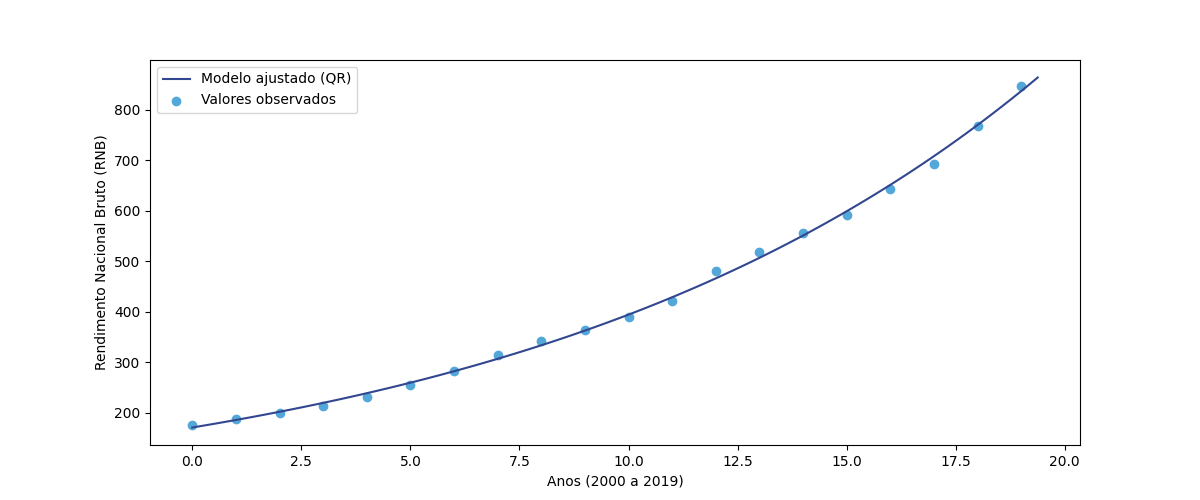
\includegraphics[width=1\linewidth]{realidadevsQR}

Através da análise do gráfico, verifica-se que a linha que representa o
modelo ajustado recorrendo à decomposição QR está alinhada com os
valores observados, isto é, os valores observados seguem o comportamento
da linha ajustada, o que sugere que o modelo capta efetivamente a
relação entre as variáveis.

\newpage
\section{Método de Levenberg-Marquardt}

Como referido anteriormente, os problemas de mínimos quadrados surgem no
contexto do ajuste de um modelo matemático parametrizado a um conjunto
de pontos fornecidos, minimizando uma função objetivo expressa como a
soma dos quadrados dos resíduos entre a função do modelo e um conjunto
de pontos dados.

\(\ \)

Dada uma função não linear nos parâmetros, o problema dos mínimos
quadrados requer um algoritmo iterativo. Tais algoritmos reduzem a soma
dos quadrados dos erros entre a função do modelo e os pontos dados
através de uma sequência de atualizações bem escolhidas nos valores dos
parâmetros do modelo. Para equações não lineares, pode não haver
solução, pode haver um qualquer número de soluções, ou um número
infinito de soluções. Ao contrário das equações lineares, é um problema
computacional muito difícil determinar qual destes casos é válido para
um determinado conjunto de equações. Assim sendo, para problemas não
lineares, apenas se pode esperar um algoritmo que encontre uma solução
(quando existe) ou produza um valor de \(x\) com norma residual que seja
a menor possível \cite{SBLV18}.

\(\ \)

O algoritmo de Levenberg-Marquardt combina dois algoritmos de
minimização numérica: o método de declive máximo e o método de
Gauss-Newton. No método de declive máximo, a soma dos erros quadráticos
é reduzida pela atualização dos parâmetros na direção de descida mais
acentuada. No método de Gauss-Newton, a soma dos erros quadráticos é
reduzida assumindo que a função de mínimos quadrados é localmente
quadrática nos parâmetros e encontrando o mínimo dessa função
quadrática.

\(\ \)

Desta forma, o nosso problema de regressão exponencial pode também ser
resolvido através deste processo, o método de Levenberg-Marquardt. Este
não envolve linearização, pelo que pode ser utilizado diretamente em
funções não lineares, o que lhe confere uma maior precisão em termos
numéricos e robustez para funções não lineares.

\(\ \)

Por conseguinte, num problema não linear de mínimos quadrados, a função
objetivo é a mesma do caso de funções lineares, e consiste na descoberta
do vetor de parâmetros \(x\) que minimiza:
\begin{equation} \label{eq:funcao_objetivo}
g(x)=\frac{1}{2}r(x)r(x)^T=\frac{1}{2}\sum_{i=1}^{m}r_i(x)^2
\end{equation}

Apesar de a função objetivo ser igual independentemente da função ser
linear ou não, os resíduos \begin{equation}
r_i(x)=y_i-f(x), \quad  i=1,...,m
\end{equation} são não lineares, tal como a função \(f(x)\).

Note-se que, o gradiente da função objetivo é dado por \begin{equation}
\nabla g(x) = \sum_{i=1}^{m}r_i(x) \cdot \nabla r_i(x) = \nabla r(x)^Tr(x)
\end{equation}

onde \begin{equation}
\nabla r(x)=\begin{bmatrix}
\frac{\partial r_1(x)}{\partial x_1} & \cdots & \frac{\partial r_1(x)}{\partial x_n} \\
\vdots &  & \vdots \\
\frac{\partial r_m(x)}{\partial x_1} & \cdots & \frac{\partial r_m(x)}{\partial x_n}
\end{bmatrix}
\end{equation} é a matriz \(m \times n\) Jacobiana do resíduo \(r\) em
relação aos parâmetros \(x\).

O vetor \begin{equation}
\nabla r_i(x)=\begin{bmatrix}
\frac{\partial r_i(x)}{\partial x_1} \\
\vdots \\
\frac{\partial r_i(x)}{\partial x_n}
\end{bmatrix}
\end{equation} corresponde à coluna \(i\) da matriz Jacobiana.

Da mesma forma, a segunda derivada de \(g(x)\) é dada pela matriz
Hessiana \begin{equation} \label{eq:hessiana}
\begin{split}
\nabla^2 g(x) & =\sum_{i=1}^{m}(\nabla r_i(x) \cdot \nabla r_i(x)^T+r_i(x) \cdot \nabla^2 r_i(x))\\
& =\nabla r(x)^T\nabla r(x) + S(x)
\end{split}
\end{equation} com \(S(x)=\sum_{i=1}^{m}r_i(x) \cdot \nabla^2 r_i(x)\)

\(\ \)

O método de Levenberg-Marquardt sugere a aproximação da matriz \(S(x)\)
pela matriz diagonal \(\mu I\) \begin{equation}
(\nabla r(x^{(k)})^T\nabla r(x^{(k)})+\mu^{(k)}I)s^{(k)}_{LM}=-\nabla r(x^{(k)})^T r(x^{(k)})
\end{equation}

A matriz \(\nabla r(x^{(k)})^T\nabla r(x^{(k)})+\mu^{(k)}I\) é simétrica
e definida positiva, \(n \times n\) (com \(n\) igual ao número de
parâmetros a estimar). Pode-se portanto, proceder à resolução do sistema
de diversas maneiras, como: a decomposição de Cholesky, a decomposição
LU, entre outras, encontrando dessa forma \(s^{(k)}_{LM}\).

O vetor dos parâmetros \(x\) será atualizado mediante cada iteração da
seguinte forma \cite{MGDMES11}, \begin{equation}
x^{(k+1)}=x^{(k)}+s^{(k)}_{LM}
\end{equation}

A cada iteração, o valor de \(x^{(k+1)}\) estará mais próximo do valor
ótimo (aquele que minimiza a soma dos quadrados), pelo que se deve
definir uma condição de paragem, podendo esta ser a quantidade de
iterações, um valor máximo para a norma do gradiente da função objetivo,
\(\|\nabla g(x)\|\), ou um valor máximo para o erro, sendo o erro
calculado por exemplo por \(\|s^{(k+1)}_{LM}\|_{\infty}\). Desta forma,
quando é alcançada a precisão desejada o processo iterativo é
interrompido, evitando assim iterações desnecessárias e economizando
recursos computacionais.

Note-se que o método LM é um método iterativo para otimização não
linear, pelo que é imperativo o fornecimento de uma aproximação inicial
dos parâmetros do modelo para uma inicialização adequada das iterações
do algoritmo.

\newpage
\subsection{Implementação em Python} \label{LM_python}

As ideias acima apresentadas podem ser sintetizadas através do seguinte
algoritmo:

\begin{Shaded}
\begin{Highlighting}[]
\ImportTok{import}\NormalTok{ numpy }\ImportTok{as}\NormalTok{ np}

\KeywordTok{def}\NormalTok{ LM\_iteration(X, Y, ig, miu):}
    \CommentTok{"""}
\CommentTok{    entrada:}
\CommentTok{        X,Y {-} conjunto de pontos}
\CommentTok{        ig, miu {-} aproximacao inicial (b0, b1), parametro mu}
\CommentTok{    saida:}
\CommentTok{        b0, b1 {-} coeficientes atualizados}
\CommentTok{    """}
\NormalTok{    matrix\_r }\OperatorTok{=}\NormalTok{ np.zeros((}\BuiltInTok{len}\NormalTok{(X), }\DecValTok{1}\NormalTok{))  }\CommentTok{\# matriz dos residuos (R)}
\NormalTok{    grad\_r }\OperatorTok{=}\NormalTok{ np.zeros((}\BuiltInTok{len}\NormalTok{(X), }\DecValTok{2}\NormalTok{))  }\CommentTok{\# gradiente de R}

\NormalTok{    b0, b1 }\OperatorTok{=}\NormalTok{ ig}
    \CommentTok{\# atualizar matrizes}
    \ControlFlowTok{for}\NormalTok{ row }\KeywordTok{in} \BuiltInTok{range}\NormalTok{(}\BuiltInTok{len}\NormalTok{(X)):}
\NormalTok{        matrix\_r[row, }\DecValTok{0}\NormalTok{] }\OperatorTok{=}\NormalTok{ Y[row] }\OperatorTok{{-}}\NormalTok{ b0 }\OperatorTok{*}\NormalTok{ np.exp(b1 }\OperatorTok{*}\NormalTok{ X[row])}

\NormalTok{        grad\_r[row, }\DecValTok{0}\NormalTok{] }\OperatorTok{=} \OperatorTok{{-}}\NormalTok{np.exp(b1 }\OperatorTok{*}\NormalTok{ X[row])  }\CommentTok{\# r gradiente: col. 1}
\NormalTok{        grad\_r[row, }\DecValTok{1}\NormalTok{] }\OperatorTok{=} \OperatorTok{{-}}\NormalTok{b0 }\OperatorTok{*}\NormalTok{ X[row]}\OperatorTok{*}\NormalTok{ np.exp(b1 }\OperatorTok{*}\NormalTok{ X[row])  }\CommentTok{\# r gradiente: col. 2}

    \CommentTok{\# calcular A(s\_LM) = b}
\NormalTok{    A }\OperatorTok{=}\NormalTok{ np.dot(grad\_r.T, grad\_r) }\OperatorTok{+}\NormalTok{ np.eye(}\DecValTok{2}\NormalTok{) }\OperatorTok{*}\NormalTok{ miu}
\NormalTok{    b }\OperatorTok{=} \OperatorTok{{-}}\NormalTok{np.dot(grad\_r.T, matrix\_r)}

    \CommentTok{\# resolver s\_LM atraves Cholesky}
\NormalTok{    L }\OperatorTok{=}\NormalTok{ np.linalg.cholesky(A)}
\NormalTok{    s\_LM\_y }\OperatorTok{=}\NormalTok{ np.linalg.solve(L, b)}
\NormalTok{    s\_LM }\OperatorTok{=}\NormalTok{ np.linalg.solve(L.T, s\_LM\_y)}

    \CommentTok{\# atualizar betas}
\NormalTok{    b0, b1 }\OperatorTok{=} \BuiltInTok{float}\NormalTok{(b0 }\OperatorTok{+}\NormalTok{ s\_LM[}\DecValTok{0}\NormalTok{]), }\BuiltInTok{float}\NormalTok{(b1 }\OperatorTok{+}\NormalTok{ s\_LM[}\DecValTok{1}\NormalTok{])}

    \ControlFlowTok{return}\NormalTok{ b0, b1, s\_LM}
\end{Highlighting}
\end{Shaded}

\newpage
\subsubsection{Exemplo - Regressão Exponencial: Problema Não Linear (LM)} \label{LM_exemplo}

Considerando o mesmo conjunto de pontos utilizado na decomposição QR,
efetua-se agora uma abordagem diferente do mesmo, recorrendo ao método
de Levenberg-Marquardt.

\begin{table}[h]
\centering
\begin{tabular}{c|ccccccccccc}
\hline
\textbf{\(x_i\)} & 0 & 1 & 2 & 3 & 4 & 5 & 6 & 7 & 8 & 9 \\
\textbf{\(y_i\)} & 175.5 & 188.1 & 200.2 & 213.7 & 231.6 & 254.7 & 283.1 & 313.5 & 342.9 & 363.7  \\
\hline
\end{tabular}
\end{table}

\begin{table}[h]
\centering
\begin{tabular}{c|ccccccccccc}
\hline
\textbf{\(x_i\)} & 10 & 11 & 12 & 13 & 14 & 15 & 16 & 17 & 18 & 19 \\
\textbf{\(y_i\)} & 389.1 & 422.2 & 481.1 & 518.8 & 555.1 & 591.6 & 643.1 & 693.0  & 767.3 & 846.1 \\
\hline
\end{tabular}
\end{table}

O vetor dos parâmetros ótimos será encontrado por aplicação do algoritmo
elaborado na secção \ref{LM_python}.

\begin{Shaded}
\begin{Highlighting}[]
\NormalTok{x }\OperatorTok{=} \BuiltInTok{list}\NormalTok{(}\BuiltInTok{range}\NormalTok{(}\DecValTok{19} \OperatorTok{+} \DecValTok{1}\NormalTok{))}
\NormalTok{y }\OperatorTok{=}\NormalTok{ [}\FloatTok{175.5}\NormalTok{, }\FloatTok{188.1}\NormalTok{, }\FloatTok{200.2}\NormalTok{, }\FloatTok{213.7}\NormalTok{, }\FloatTok{231.6}\NormalTok{, }\FloatTok{254.7}\NormalTok{, }\FloatTok{283.1}\NormalTok{, }\FloatTok{313.5}\NormalTok{, }\FloatTok{342.9}\NormalTok{, }\FloatTok{363.7}\NormalTok{, }\FloatTok{389.1}\NormalTok{, }\FloatTok{422.2}\NormalTok{,}
    \FloatTok{481.1}\NormalTok{, }\FloatTok{518.8}\NormalTok{, }\FloatTok{555.1}\NormalTok{, }\FloatTok{591.6}\NormalTok{, }\FloatTok{643.1}\NormalTok{, }\FloatTok{693.0}\NormalTok{, }\FloatTok{767.3}\NormalTok{, }\FloatTok{846.1}\NormalTok{]}

\NormalTok{ig }\OperatorTok{=}\NormalTok{ (}\DecValTok{170}\NormalTok{, }\FloatTok{0.0836}\NormalTok{) }\CommentTok{\#obtido atraves do exemplo da seccao 2.3.3}
\NormalTok{miu }\OperatorTok{=} \FloatTok{0.1}

\NormalTok{iteracoes }\OperatorTok{=} \DecValTok{1}
\ControlFlowTok{while} \VariableTok{True}\NormalTok{:}
\NormalTok{    b0, b1, s\_LM }\OperatorTok{=}\NormalTok{ LM\_iteration(x, y, ig, miu)}

    \CommentTok{\# condicao de paragem}
    \ControlFlowTok{if} \BuiltInTok{max}\NormalTok{(}\BuiltInTok{abs}\NormalTok{(s\_LM)) }\OperatorTok{\textless{}} \FloatTok{0.5}\OperatorTok{*}\DecValTok{10}\OperatorTok{**}\NormalTok{(}\OperatorTok{{-}}\DecValTok{6}\NormalTok{):}
            \ControlFlowTok{break}
    
    \CommentTok{\# atualizar parametros}
\NormalTok{    ig }\OperatorTok{=}\NormalTok{ (b0, b1)}
\NormalTok{    miu }\OperatorTok{=} \FloatTok{0.1}
\NormalTok{    iteracoes }\OperatorTok{+=} \DecValTok{1}

\NormalTok{iteracoes, b0, b1}
\end{Highlighting}
\end{Shaded}

\begin{verbatim}
## (4, 171.5072875301047, 0.08333471235500428)
\end{verbatim}

Assim, após o algoritmo de Levenberg-Marquardt realizar 4 iterações, a
função que minimiza os quadrados dos resíduos, de acordo com o mesmo, é
dada por aproximadamente \(y = 171.5\ e^{0.08333x}\).

\(\ \)

Podemos confirmar este resultado através da aplicação da função
\textit{nls}: Nonlinear Least Squares, do R. É necessário indicar o
nosso conjunto de pontos e uma aproximação inicial, tal como no método
LM, sendo que a única diferença é o parâmetro \(\mu\) ter um valor nulo,
pelo que o método utilizado por esta função é o método de Gauss-Newton.
Ao utilizar-se os mesmos dados definidos acima, tem-se que:

\begin{Shaded}
\begin{Highlighting}[]
\FunctionTok{nls}\NormalTok{(y }\SpecialCharTok{\textasciitilde{}}\NormalTok{ b0}\SpecialCharTok{*}\FunctionTok{exp}\NormalTok{(b1}\SpecialCharTok{*}\NormalTok{x), }\AttributeTok{start =} \FunctionTok{list}\NormalTok{(}\AttributeTok{b0 =} \DecValTok{170}\NormalTok{, }\AttributeTok{b1 =} \FloatTok{0.0836}\NormalTok{))}
\end{Highlighting}
\end{Shaded}

\begin{verbatim}
## Nonlinear regression model
##   model: y ~ b0 * exp(b1 * x)
##    data: parent.frame()
##        b0        b1 
## 171.50728   0.08333 
##  residual sum-of-squares: 1159
## 
## Number of iterations to convergence: 2 
## Achieved convergence tolerance: 4.694e-07
\end{verbatim}

Note-se que os resultados são aproximadamente iguais, mas tendo em conta
o número de iterações, a escolha do valor do parâmetro \(\mu\) terá sido
conservadora, levando a uma otimização mais lenta.

\(\ \)

Por fim, tal como efetuado para o exemplo relativo à decomposição QR,
procede-se à representação gráfica dos valores observados em conjunto
com o modelo ótimo estimado.

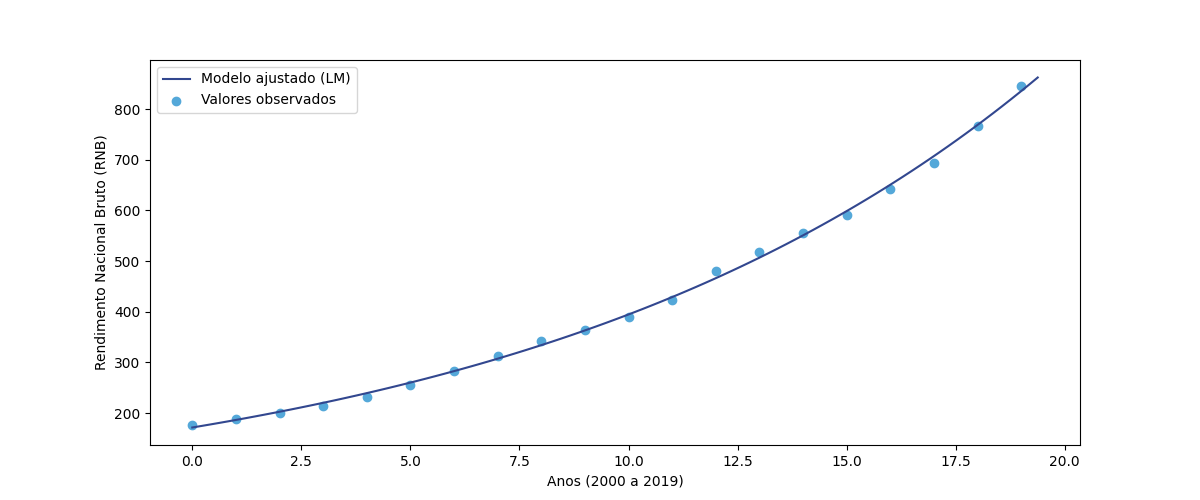
\includegraphics[width=1\linewidth]{realidadevsLM}

Através da análise do gráfico, verifica-se que a linha que representa o
modelo ajustado recorrendo ao método de Levenberg-Marquardt está
alinhada com os valores observados, isto é, os valores observados seguem
o comportamento da linha ajustada, o que sugere que o modelo capta, de
facto, a relação entre as variáveis.

\subsection{Escolha da aproximação inicial}

É importante recordar que o método de Levenberg-Marquardt não garante a
descoberta do mínimo global. O sucesso da resolução do problema de
otimização irá depender da natureza do problema e da qualidade da
aproximação inicial escolhida, pelo que se torna essencial uma análise
específica do problema.

Ou seja, caso a aproximação inicial esteja muito longe do mínimo global,
o algoritmo pode convergir para um mínimo local, uma solução que é ótima
dentro de uma determinada vizinhança, mas pode não ser o ótimo global
para toda a região de parâmetros \cite{GZDAJC20}. Isto pode ser
resolvido através da seleção de uma aproximação inicial próxima da
solução esperada, o que muitas vezes implica um conhecimento à priori ou
uma análise minuciosa dos dados.

Por isso, a escolha da aproximação inicial é um passo muito importante
no método LM, podendo impactar significativamente a convergência e o
resultado final da otimização.

Uma boa aproximação inicial fornece ao algoritmo um ponto de partida
próximo da solução ótima, permitindo uma convergência mais rápida. Por
outro lado, uma aproximação inicial inadequada, que esteja muito longe
do mínimo global, leva a uma convergência lenta, aumentando o número de
iterações necessárias e a exigência computacional. Para além disso, pode
levar o algoritmo a convergir para um mínimo local ou a falhar na
convergência.

Apesar de haverem diversos métodos para se obter uma aproximação inicial
para o algoritmo, os dois mais comuns são a utilização dos resultados de
aproximações lineares, ou seja, aproximar o modelo a um linear e estimar
o resultado que minimiza os quadrados dos resíduos, por exemplo através
da utilização da decomposição QR (tal como na secção
\ref{exp_aplicado_qr}), ou então por tentativa e erro, isto é, executar
o algoritmo de otimização várias vezes com diferentes aproximações
iniciais aleatórias, explorando diferentes regiões do espaço de
parâmetros, e compararando as mesmas, de modo a reduzir o risco de se
obter um mínimo local e não global \cite{GZDAJC20}.

\subsection{Escolha do parâmetro $\mu$}

O valor do parâmetro \(\mu\), frequentemente chamado de termo de
amortecimento, no algoritmo de Levenberg-Marquardt, impacta diretamente
o termo \(\mu I\), regularizando a matriz Hessiana (\ref{eq:hessiana})
durante a sua inversão, para o cálculo da atualização dos parâmetros do
modelo durante a otimização, tornando-a mais estável numericamente
\cite{MCYZBXXG17}.

Assim, a seleção apropriada do valor para o parâmetro \(\mu\) desempenha
um papel crucial no comportamento do algoritmo de Levenberg-Marquardt,
pelo que a sua escolha deve ser cuidada.

Caso o valor de \(\mu\) seja pequeno (\(\mu \rightarrow 0\)), o
algoritmo de Levenberg-Marquardt assemelha-se ao método de Gauss-Newton
\cite{SBLV18}. Nesse cenário, a atualização dos parâmetros tem uma maior
ponderação da matriz Jacobiana, tornando o processo de otimização menos
cuidadoso, o que resulta numa convergência mais rápida (caracterizada
por um menor número de iterações). Esta abordagem é particularmente
eficaz quando o modelo é bem comportado e a aproximação inicial está
próxima da solução ótima.

Quando o valor de \(\mu\) é grande (\(\mu \rightarrow \infty\)), o
comportamento do algoritmo de Levenberg-Marquardt aproxima-se do método
de declive máximo \cite{PC07}. Nesse caso, \(\mu I\) torna-se dominante
na atualização dos parâmetros, o que resulta num processo de otimização
mais cuidadoso em que \(x^{(k+1)}\) está próximo de \(x^{(k)}\),
aumentando a estabilidade numérica do algoritmo. Esta abordagem é
vantajosa ao lidar com modelos mal comportados.

\(\ \)

Visualize-se graficamente o impacto da escolha do valor de \(\mu\) na
resolução do exemplo \ref{LM_exemplo}. Note-se que a aproximação inicial
é (\(168\), \(0.0825\)) e o parâmetro \(\mu\) irá assumir dois valores:
um valor grande (\(\mu = 100\)) e um valor pequeno (\(\mu = 0.01\)):

\(\ \)

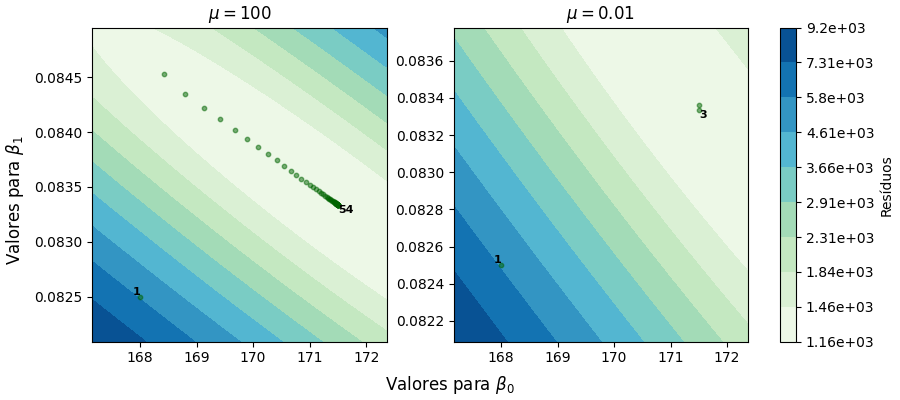
\includegraphics[width=1\linewidth]{LM_miu}

Verifica-se que para \(\mu=100\) o algoritmo realiza 54 iterações até
verificar a condição de paragem de
\(\|s^{(k)}_{LM}\|_{\infty}<0.5 \times 10^{-3}\), enquanto que com
\(\mu=0.01\) o mesmo apenas realiza 3 iterações.

\(\ \)

Pode-se notar então que a escolha do valor para \(\mu\) envolve um
equilíbrio entre a velocidade de convergência e a estabilidade numérica
do algoritmo, pelo que a sua escolha deve ter em conta as
características específicas do problema, não sendo escolhido de forma
arbitrária.

Existem várias variações do método de Levenberg-Marquardt onde se podem
verificar diferentes abordagens para a escolha do parâmetro \(\mu\).
Algumas publicações indicam que o parâmetro deve ser escolhido pelo
utilizador do algoritmo \cite{DM63}, outras indicam que o mesmo deve ser
atualizado a cada iteração de acordo com o valor de
\(\| \nabla r(x^{(k)})' r(x^{(k)}) \|\) \cite{LCYM23}, há quem indique
que se deve começar com um valor pequeno para o parâmetro e dividir ou
multiplicar por 10 caso a função objetivo melhore ou piore,
respetivamente \cite{PC07}, etc.

Contudo, verifica-se que o comum é o valor do parâmetro \(\mu\) ser
ajustado de acordo com o progresso da otimização, isto é, se a iteração
realizada melhorar o valor da função objetivo, o valor de \(\mu\) pode
ser reduzido para permitir o algoritmo convergir mais rapidamente, caso
contrário, o seu valor deve ser aumentado {[}Nocedal and Wright,
2006{]}. \textcolor{white}{\cite{JNSW06}}

Assim sendo, o método de Levenberg-Marquardt deve atuar mais como o
método de declive máximo quando os parâmetros estão longe do seu valor
ótimo, e atuar mais como o método de Gauss-Newton quando os parâmetros
estão próximos do mesmo \cite{HPG22}.

\newpage
\section{Conclusão}

A realização deste trabalho permitiu a análise da eficiência e da
confiabilidade de duas técnicas fundamentais: a decomposição QR e o
método de Levenberg-Marquardt, na estimativa de parâmetros para modelos
matemáticos, nomeadamente, modelos exponenciais.

\(\ \)

Note-se que é de elevada importância relembrar os resultados dos
exemplos associados à decomposição QR (secção \ref{QR_exemplo}) e ao
método de Levenberg-Marquardt (secção \ref{LM_exemplo}). Enquanto que no
exemplo associado à decomposição QR se obteve o vetor de parâmetros
(\(171.0\), \(0.08356\)), no exemplo associado ao método LM o vetor de
parâmetros obtido foi (\(171.5\), \(0.08333\)). Por isso, devemos
analisar o valor ótimo da função objetivo \ref{eq:funcao_objetivo} para
cada vetor de parâmetros:

\begin{Shaded}
\begin{Highlighting}[]
\KeywordTok{def}\NormalTok{ funcao\_objetivo(y,x,beta):}
\NormalTok{    r\_i }\OperatorTok{=}\NormalTok{ y }\OperatorTok{{-}}\NormalTok{ beta[}\DecValTok{0}\NormalTok{]}\OperatorTok{*}\NormalTok{np.exp(beta[}\DecValTok{1}\NormalTok{]}\OperatorTok{*}\NormalTok{x)}
\NormalTok{    valor\_otimo }\OperatorTok{=} \FloatTok{0.5} \OperatorTok{*}\NormalTok{ np.}\BuiltInTok{sum}\NormalTok{(r\_i}\OperatorTok{**}\DecValTok{2}\NormalTok{)}
    \ControlFlowTok{return}\NormalTok{ valor\_otimo}

\NormalTok{beta\_QR, beta\_LM }\OperatorTok{=}\NormalTok{ (}\FloatTok{171.0}\NormalTok{, }\FloatTok{0.08356}\NormalTok{), (}\FloatTok{171.5}\NormalTok{, }\FloatTok{0.08333}\NormalTok{)}
\NormalTok{funcao\_objetivo(y,x,beta\_QR), funcao\_objetivo(y,x,beta\_LM)}
\end{Highlighting}
\end{Shaded}

\begin{verbatim}
## (582.0077304979613, 579.6157244799521)
\end{verbatim}

Verifica-se que o valor ótimo obtido pelos parâmetros associados à
decomposição QR é superior ao valor ótimo obtido pelos parâmetros
associados método de Levenberg-Marquardt (\(582.0 > 579.6\)), pelo que o
método LM efetuou uma otimização mais precisa face à associada à
decomposição QR, dado que é um problema de minimização.

Visto que ambas as técnicas têm em conta o método dos mínimos quadrados,
esta diferença nos resíduos estará associada à precisão numérica da
técnica, isto é, pelo facto do algoritmo LM ser de aplicação direta,
enquanto que para aplicar a decomposição QR, têm de ser realizadas
diversas operações para linearizar a função e só depois a aplicação da
própria decomposição. Era portanto expectável que a precisão associada à
decomposição QR na estimação dos parâmetros fosse menor, devido à
propagação do erro.

\(\ \)

A pesquisa sobre a decomposição QR demonstra a sua eficácia, já
conhecida, na resolução de sistemas de equações lineares. Através da
decomposição da matriz dos coeficientes dos parâmetros a estimar numa
matriz ortogonal e numa matriz triangular superior, é possível a
agilização do processo de descoberta do vetor de parâmetros ótimo. Este
processo torna-se particularmente benéfico quando estamos perante
sistemas lineares de maior dimensão.

Contudo, considerando modelos exponenciais, pelo facto de ser necessário
linearizar o modelo, a decomposição QR é afetada pela propagação do
erro, pelo que se pode chegar a um vetor de parâmetros que não
corresponde ao ótimo, logo é importante proceder a uma análise crítica
dos resultados e considerar métodos de otimização mais avançados.

\(\ \)

De qualquer forma, a utilização desta técnica pode ser extremamente útil
para se obter uma aproximação inicial para métodos iterativos como é o
caso da segunda técnica utilizada, o método LM.

\(\ \)

Tendo em conta o método de Levenberg-Marquardt, pode-se verificar que
este é uma interpolação entre o método de Gauss-Newton e o método de
declive máximo, ainda que mais robusto que o primeiro. Percebe-se isto
quando, na maioria dos casos, é possível obter uma solução mesmo quando
se parte de um ponto muito longe do mínimo ótimo, ainda que mais
lentamente que o método de Gauss-Newton.

Para além disso, ao analisar os resultados do exemplo relativo a este
método, verifica-se que os mesmos demonstram a eficácia do método LM em
explorar regiões não lineares nos espaços dos parâmetros, convergindo
para soluções ótimas, tornando o método uma ferramenta valiosa para a
estimação de parâmetros ótimos em modelos não lineares, nomeadamente
modelos exponenciais, destacando a sua robustez e adaptabilidade.

\newpage
\bibliographystyle{apalike}
\bibliography{refs}
\addcontentsline{toc}{section}{Referências}


\end{document}
